%%%%%%%%%%%%%%%%%%%%%%%%%%%%%%%%%%%%%%%%%%%%%%%%%%%%%%%%%%%%%%%%%%%%%%%%%%%%%%%%
% Timer
%%%%%%%%%%%%%%%%%%%%%%%%%%%%%%%%%%%%%%%%%%%%%%%%%%%%%%%%%%%%%%%%%%%%%%%%%%%%%%%%
\chapter{Timer} \label{Timer}
\vspace{-10ex}\mTi{syml}\vskip 8ex

%%%%%%%%%%%%%%%%%%%%%%%%%%%%%%%%%%%%%%%%%%%%%%%%%%%%%%%%%%%%%%%%%%%%%%%%%%%%%%%%
% Introduction
%%%%%%%%%%%%%%%%%%%%%%%%%%%%%%%%%%%%%%%%%%%%%%%%%%%%%%%%%%%%%%%%%%%%%%%%%%%%%%%%
\section{Introduction}

Allows setting and running a timer.  The timer can be set anywhere from \num{1}
second to \num{99} hours and \num{99} minutes, can be paused using the \cEs{f}
and alerts when the timer expires using the \cBe{f} that can be turned off using
either the \cEs{f} or \aTo{f}.

\par\medskip

There is also the option, by touching the top of the enclosure for \num{1}
second, to toggle the use of the \cLi{f} window as a display of colors that
change as the timer counts down giving a visual indication as to the approximate
time left.

\par\medskip

The clock can also be displayed while the timer is active by using the \cEs{f}.

\par\medskip

There are a few ways to get to \mTi{f} mode depending on which direction the
\cRs{f} is pointing and which mode the device is currently in.

\ers{2.3}
\begin{table}[H]
  \centering
  \begin{tabu} { X[1,c,m] | X[1,c,m] | X[1,c,m] }
    \thrule
    \thbi{Position} & \thbi{Mode} & \thbi{Action} \\ \mrule

    \sLe & \multirow{2}{*}[-1mm]{\mode{s}{ANY}} & \sLtoR \\ \dcrule{1}{1} \dcrule{3}{3}
    \sMi & & $\hskip 4mm$ \sMtoR \\ \mdrule

    \multirow{4}{*}[-9mm]{\sRi}
      & \mPS{sym} & \sSec \\ \dcrule{2}{3}

    & \multirow{2}{*}[-1.5mm]{\mSN{sym}}
      & \sSec \\ \dcrule{3}{3}
    & & \sTer \\ \dcrule{2}{3}

    & \mode{f}{ANY} & \sRtoM \quad\quad \sMtoR \\

    \bhrule
  \end{tabu}
  \caption{Timer - Mode}
\end{table}

%%%%%%%%%%%%%%%%%%%%%%%%%%%%%%%%%%%%%%%%%%%%%%%%%%%%%%%%%%%%%%%%%%%%%%%%%%%%%%%%
% Overview
%%%%%%%%%%%%%%%%%%%%%%%%%%%%%%%%%%%%%%%%%%%%%%%%%%%%%%%%%%%%%%%%%%%%%%%%%%%%%%%%
\section{Overview}

There are a number of states \mTi{f} can be in and are explained in the next
sections.

\ers{2}
\begin{table}[H]
  \centering
  \begin{tabu} { X[1,c,m] | X[3,l,m] }
    \thrule
    \thbi{State} & \thbi{Description} \\ \mrule

    \sTiHM{sym} & Set hours | minutes field. \\ \drule{2}
    \sTiMS{sym} & Set minutes if \sTiHM{f} is in hours or
      seconds if in minutes.  \\ \drule{2}
    \sTiRu{sym} & Timer is actively counting down.  \\ \drule{2}
    \sTiPa{sym} & Timer countdown is paused.  \\ \drule{2}
    \sTiAl{sym} & Timer expired and is alerting\slash beeping.  \\ \drule{2}
    \sTiWa{sym} & State after alerting is stopped or first state if
        a time has previously been set. \\
    \bhrule
  \end{tabu}
  \caption{Timer - States}
\end{table}

The first time \mTi{f} is entered after the device is switched \sOn{f}, the
time will have to be set and the first state will be \sTiHM{f}.  The general
progression involves first, setting the time, after which the timer starts
running, then letting the timer count down to \num{0} at which time it begins
alerting, and then stopping the alerting by either \action{f}{TURNING} the
\cEs{f} or \action{f}{TOUCHING} the \control{f}{TOP} of the enclosure.

\tabcolsep=10pt
\ase{1}{{c c c c c c c c c c c}}{%
\multirow{2}{*}{\sTiHM{sym}}
  & \multirow{2}{*}{\sTu}
  & \multirow{2}{*}{\sPR}
  & \multirow{2}{*}{\sTiMS{sym}}
  & \multirow{2}{*}{\sTu}
  & \multirow{2}{*}{\sPR}
  & \multirow{2}{*}{\sTiRu{sym}}
  & \multirow{2}{*}{\eAc{sym}{TIMER EXPIRES}}
  & \multirow{2}{*}{\sTiAl{sym}}
  & \sPR
  & \multirow{2}{*}{\sTiWa{sym}} \\ \dcrule{10}{10}
& & & & & & & & & \sTo & \\}
\tabcolsep=12pt

\info{For touch to work, make sure you have enabled it via
\hyperref[Touch Settings]{\mTS{f}} and that the palm of your hand or
most of your fingers touch the top of the enclosure - it won't likely be enough
to just touch or tap the top with one finger.}

Subsequent entries into \mTi{f} mode will load the previously set time and the
first state will be \sTiWa{f}\footnote{ The time isn't saved when the device is
powered \sOff{f} via the \cPo{ss} switch, so each time the device is powered
\sOn{f} it will start in \sTiHM{ss} state and you will have to set the time.}
from which you can either start the timer by pressing and releasing the \cEs{f}.

\as{{c c c c c}}{\mTi{sym} & \sTiWa{sym} & \sPR & \sTiRu{sym} & $\cdots$ \\}

or set a new time by turning the \cEs{f}.

\as{{c c c c c}}{\mTi{sym} & \sTiWa{sym} & \sTu & \sTiMS{sym} & $\cdots$ \\}

When the timer is running, you can \sTiPa{f} it by a \aPR{f} of the \cEs{f}.
To resume, \aPR{f} again.

\as{{c c c c c c}}{\sTiRu{sym} & \sPR & \sTiPa{sym} & \sPR & \sTiRu{sym} & $\cdots$ \\}

%%%%%%%%%%%%%%%%%%%%%%%%%%%%%%%%%%%%%%%%%%%%%%%%%%%%%%%%%%%%%%%%%%%%%%%%%%%%%%%%
% Set Time
%%%%%%%%%%%%%%%%%%%%%%%%%%%%%%%%%%%%%%%%%%%%%%%%%%%%%%%%%%%%%%%%%%%%%%%%%%%%%%%%
\section{Set Time}

Setting the time occurs on one screen of the \cDi{f} and is composed of two
states - \sTiHM{f} and \sTiMS{f}. The current setting, first \sTiHM{f}, then
\sTiMS{f}, will be \textit{blinking}.  The time can be set anywhere from \num{1}
second to \num{99} hours and \num{99} minutes.

\figDT{00:01}{1 Second}{99:99.}{99 Hours \& 99 Minutes}

To the \textit{left} of the \textit{colon} is where you set the minutes or if
more than \num{59} minutes, the hours.  As you \aTu{f} the \cEs{f}
\textit{clockwise} the number will increase until it hits \num{59} minutes at
which point it will change over to hours and display a \textit{decimal} in the
\textit{lower right} of the \cDi{f}.  The decimal indicates that the time is in
hours and minutes or \mono{HH:MM}.

\figDT{59:00}{59 Minutes}{!1:00.}{1 Hour}

Like other options, the numbers in the fields will wrap.  Below shows the basic
milestones as you turn in one direction or the other when in \sTiHM{f}.

\ase{1}{{c c c c c c c c}}{%
\sCl & \sD{!0:00} & $\cdots$ & \sD{59:00}
  & \sD{!1:00.} & $\cdots$ & \sD{99:00.} & \sD{!0:00} \\ \drule{8}
\sCC & \sD{!0:00} & \sD{99:00.} & $\cdots$
  & \sD{!1:00.} & \sD{59:00} & $\cdots$ & \sD{!0:00} \\}

%%%%%%%%%%%%%%%%%%%%%%%%%%%%%%%%%%%%%%%%%%%%%%%%%%%%%%%%%%%%%%%%%%%%%%%%%%%%%%%%
% Set Time - Set H|M
%%%%%%%%%%%%%%%%%%%%%%%%%%%%%%%%%%%%%%%%%%%%%%%%%%%%%%%%%%%%%%%%%%%%%%%%%%%%%%%%
\subsection{Set Hours or Minutes} \sTiHM{syml}

Set the hours or minutes.

\par\medskip

To select the hours or minutes, \aTu{f} the \cEs{f} then \aPR{f} to cache the
setting and move on to \sTiMS{f}.

\as{{c c c c}}{%
\multirow{2}{*}{\sTiHM{sym}}
  & \sTu & \sPR & \multirow{2}{*}{\sTiMS{sym}} \\
& \eUp{sym}{} & \eCa{sym}{} & \\}

%%%%%%%%%%%%%%%%%%%%%%%%%%%%%%%%%%%%%%%%%%%%%%%%%%%%%%%%%%%%%%%%%%%%%%%%%%%%%%%%
% Set Time - Set M|S
%%%%%%%%%%%%%%%%%%%%%%%%%%%%%%%%%%%%%%%%%%%%%%%%%%%%%%%%%%%%%%%%%%%%%%%%%%%%%%%%
\subsection{Set Minutes or Seconds} \sTiMS{syml}

Set the minutes or seconds.

\par\medskip

To select the minutes or seconds, \aTu{f} the \cEs{f} then \aPR{f} to start the
timer.

\as{{c c c c}}{%
\multirow{2}{*}{\sTiMS{sym}}
  & \sTu & \sPR & \multirow{2}{*}{\sTiRu{sym}} \\
& \eUp{sym}{} & \eStart{sym}{TIMER} & \\}

%%%%%%%%%%%%%%%%%%%%%%%%%%%%%%%%%%%%%%%%%%%%%%%%%%%%%%%%%%%%%%%%%%%%%%%%%%%%%%%%
% Run
%%%%%%%%%%%%%%%%%%%%%%%%%%%%%%%%%%%%%%%%%%%%%%%%%%%%%%%%%%%%%%%%%%%%%%%%%%%%%%%%
\section{Run} \sTiRu{syml}

Timer is actively counting down.

\par\medskip

As the timer is actively counting down, the \cDi{f} is updated every second.

\begin{itemize}[leftmargin=*]
  \item If the time left is \textit{less} than \num{1} hour, the time will be
    formatted as minutes and seconds - \mono{MM:SS} - and progress can easily be
    seen as the seconds count down.
  \item Otherwise, when the time left is \num{1} hour or greater, since the time
    will be formatted as hours and minutes - \mono{HH:MM} - the \textit{decimal}
    in the \textit{lower right} of the \cDi{f} will \textit{blink} on and off
    every second to give an indication of progress.
\end{itemize}

To stop the timer before it has finished counting down, perform a \aReset{f},
i.e. \aPH{f} the \cEs{s} until \symD{<<<<} is blinking on the \cDi{f}.  This
can also be done in the \sTiPa{f} state.

\ase{1}{{c c c c}}{%
\sTiRu{sym} & \multirow{2}{*}{\sReset}
  & \multirow{2}{*}{\eSt{sym}{TIMER}}
  & \multirow{2}{*}{\sTiWa{sym}} \\ \dcrule{1}{1}
\sTiPa{sym} & & & \\}

When the timer expires, it will begin alerting with the \cBe{f}.

\ase{1}{{c c c c}}{\sTiRu{sym} & \eAc{sym}{TIMER EXPIRES} & \sTiAl{sym} \\}

%%%%%%%%%%%%%%%%%%%%%%%%%%%%%%%%%%%%%%%%%%%%%%%%%%%%%%%%%%%%%%%%%%%%%%%%%%%%%%%%
% Run - Lighting
%%%%%%%%%%%%%%%%%%%%%%%%%%%%%%%%%%%%%%%%%%%%%%%%%%%%%%%%%%%%%%%%%%%%%%%%%%%%%%%%
\subsection{Lighting} \label{Timer - Lighting}

The \cLi{f} window will be lit and progress seamlessly through the following
primary hues as the timer counts down giving a visual indication as to the
approximate time left.

\begin{table}[H] \ers{0.1} \begin{tabu} { c }
\cBl \cGr \cYe \cOr \cRe
\end{tabu} \end{table}

This is useful if you are some distance from the device and can't see the time
on the \cDi{f} or in a dimly lit or dark area and not facing the \cDi{f}.
However, if you don't want the lighting on while the timer is counting down,
it can be turned off.

\par\medskip

To toggle between showing and not showing the colors in the \cLi{f} window,
\aTo{f} the \cTo{f} of the enclosure for \num{1} second.  This can also be done
in the \sTiPa{f} state.

\ase{1}{{c c c}}{%
\sTiRu{sym} & \multirow{2}{*}{\sToN{1}}
  & \multirow{2}{*}{\eTo{sym}{LIGHTING ON|OFF}} \\ \dcrule{1}{1}
\sTiPa{sym} & & \\}

\info{For touch to work, make sure you have enabled it via
\hyperref[Touch Settings]{\mTS{f}} and that the palm of your hand or most of
your fingers lay on top of the enclosure.}

%%%%%%%%%%%%%%%%%%%%%%%%%%%%%%%%%%%%%%%%%%%%%%%%%%%%%%%%%%%%%%%%%%%%%%%%%%%%%%%%
% Pause
%%%%%%%%%%%%%%%%%%%%%%%%%%%%%%%%%%%%%%%%%%%%%%%%%%%%%%%%%%%%%%%%%%%%%%%%%%%%%%%%
\section{Pause} \sTiPa{syml}

Timer is paused.

\par\medskip

When the timer is counting down, i.e. in the \sTiRu{f} state, you can pause it.
To toggle between the \sTiRu{f} and \sTiPa{f} states, \aPR{f} the \cEs{f}.

\as{{c c c c c}}{%
\multirow{2}{*}{\sTiRu{sym}}
  & \sPR & \multirow{2}{*}{\sTiPa{sym}} & \sPR & \multirow{2}{*}{\sTiRu{sym}} \\
& \ePa{sym}{TIMER} & & \eResume{sym}{TIMER} & \\}

%%%%%%%%%%%%%%%%%%%%%%%%%%%%%%%%%%%%%%%%%%%%%%%%%%%%%%%%%%%%%%%%%%%%%%%%%%%%%%%%
% Alert
%%%%%%%%%%%%%%%%%%%%%%%%%%%%%%%%%%%%%%%%%%%%%%%%%%%%%%%%%%%%%%%%%%%%%%%%%%%%%%%%
\section{Alert} \sTiAl{syml}

The timer has expired and is alerting.

\par\medskip

When the timer expires, the \cBe{f} will alert and both the \cDi{f} and \cLi{f}
will blink in sync. The \cLi{f} window will blink red if it hasn't been turned
off and the \cDi{f} will blink

\begin{figure}[H]
\centering
  \sDl{donE}
\end{figure}

You can either \aPR{f} the \cEs{f} or \aTo{f} the \cTo{f} of the enclosure to
stop the alerting.  After the alerting is stopped, the \mTi{f} will go to the
\sTiWa{f} state.

\ase{1}{{c c c c}}{%
\multirow{2}{*}{\sTiAl{sym}} & \sPR
  & \multirow{2}{*}{\eSt{sym}{ALERTING}}
  & \multirow{2}{*}{\sTiWa{sym}} \\ \dcrule{2}{2}
& \sTo & & \\}

%%%%%%%%%%%%%%%%%%%%%%%%%%%%%%%%%%%%%%%%%%%%%%%%%%%%%%%%%%%%%%%%%%%%%%%%%%%%%%%%
% Wait
%%%%%%%%%%%%%%%%%%%%%%%%%%%%%%%%%%%%%%%%%%%%%%%%%%%%%%%%%%%%%%%%%%%%%%%%%%%%%%%%
\section{Wait} \sTiWa{syml}

Wait for user input.

\par\medskip

This is the state the \mTi{f} enters after \sTiAl{f} or from \sTiRu{f},
\sTiPa{f} or \sTiAl{f} when \aReset{f}.  Also, if you have previously set a
time, it will be the first state upon reentering \mTi{f} mode.

\par\medskip

If you don't need to update the time, \aPR{f} the \cEs{f} and the timer will
start counting down and be in the \sTiRu{f} state.

\as{{c c c}}{%
\multirow{2}{*}{\sTiWa{sym}}
  & \sPR & \multirow{2}{*}{\sTiRu{sym}} \\
& \eStart{sym}{TIMER} & \\}

If you want to adjust the time, \aTu{f} the \cEs{f}.

\as{{c c c}}{\sTiWa{sym} & \sTu & \sTiHM{sym} \\}

%%%%%%%%%%%%%%%%%%%%%%%%%%%%%%%%%%%%%%%%%%%%%%%%%%%%%%%%%%%%%%%%%%%%%%%%%%%%%%%%
% Show Clock
%%%%%%%%%%%%%%%%%%%%%%%%%%%%%%%%%%%%%%%%%%%%%%%%%%%%%%%%%%%%%%%%%%%%%%%%%%%%%%%%
\section{Show Clock}

When in \sTiRu{f} or \sTiPa{f} states the \cDi{f} can toggle between showing the
clock time and timer countdown time. To toggle between the two, \aTu{f} the
\cEs{f} at least \num{3} \textit{detents} quickly either clockwise or
counter-clockwise.

\ase{1}{{c c c}}{%
\sTiRu{sym}
  & \multirow{2}{*}{\sTuN{3}}
  & \multirow{2}{*}{\eTo{sym}{SHOW CLOCK|TIMER}} \\ \dcrule{1}{1}
\sTiPa{sym} & & \\}

Really just a quick \aTu{f} in either direction will work.  The timer will
continue to count down and the \cLi{f} window will continue to change color in
either case, so when the clock time is displayed, you can still get a feel for
the amount of timer time left by the color in the \cLi{f} window.  When the
timer expires, it will go into the \sTiAl{f} state which will take over the
\cDi{f}.

%%%%%%%%%%%%%%%%%%%%%%%%%%%%%%%%%%%%%%%%%%%%%%%%%%%%%%%%%%%%%%%%%%%%%%%%%%%%%%%%
% Power
%%%%%%%%%%%%%%%%%%%%%%%%%%%%%%%%%%%%%%%%%%%%%%%%%%%%%%%%%%%%%%%%%%%%%%%%%%%%%%%%
\section{Power}

The screens will either \sScDi{f} or turn \sScOf{f} depending on the current
state.  If the \mTi{f} is in either \sTiRu{f} or \sTiAl{f} states, the screens
will \sDim{f} for both \sPoNa{f} and \sPoSl{f} states, however, the device will
\textit{not} go to sleep - it will instead \sPoNa{f}.  For the other \mTi{f}
states, the screens will turn \sOff{f} in both \sPoNa{f} and \sPoSl{f} power
states.

\begin{table}[H]
\ers{2}
\begin{tabu}{ X[1,c,m] | X[1,c,m] | X[1,c,m] }
  \thrule
  \thbi{Power State} & \thbi{Timer State} & \thbi{Screens} \\ \mrule

  \multirow{2}{*}[-1mm]{\sPoNa{sym}}
    & \sTiRu{sym} \sTiAl{sym} & \sDim{sym} \\ \dcrule{2}{3}
  & \sTiHM{sym} \sTiMS{sym} \sTiPa{sym} \sTiWa{sym} & \sOff{sym} \\ \mrule

  \sPoSl{sym} $\rightarrow$ \sPoNa{sym} & \sTiRu{sym} \sTiAl{sym} & \sDim{sym} \\ \mrule
  \sPoSl{sym} & \sTiHM{sym} \sTiMS{sym} \sTiPa{sym} \sTiWa{sym} & \sOff{sym} \\

  \bhrule
\end{tabu}
\caption {Timer - Power}
\end{table}

%%%%%%%%%%%%%%%%%%%%%%%%%%%%%%%%%%%%%%%%%%%%%%%%%%%%%%%%%%%%%%%%%%%%%%%%%%%%%%%%
% Reference
%%%%%%%%%%%%%%%%%%%%%%%%%%%%%%%%%%%%%%%%%%%%%%%%%%%%%%%%%%%%%%%%%%%%%%%%%%%%%%%%
\section{Reference}

\ers{2.4}
\begin{longtabu}{ X[2,c,m] | X[1,c,m] | X[4,c,m] | X[2,c,m] }
  \thrule
  \thbi{State} & \thbi{Action} & \thbi{Effect} & \thbi{Next} \\ \hline

  \multirow{2}{*}[-1.5mm]{\sTiHM{sym}}
    & \sTu & \eUp{sym}{H|M} & --- \\ \dcrule{2}{4}
  & \sPR & \eBl{sym}{M|S} & \sTiMS{sym} \\ \mrule

  \multirow{2}{*}[-1.5mm]{\sTiMS{sym}}
    & \sTu & \eUp{sym}{M|S} & --- \\ \dcrule{2}{4}
  & \sPR & \eStart{sym}{TIMER} & \sTiRu{sym} \\ \mrule

  \multirow{4}{*}[-1.5mm]{\sTiRu{sym}}
    & \sPR & \ePa{sym}{TIMER} & \sTiPa{sym} \\ \dcrule{2}{4}
  & $\hskip 1.2mm$ \sTuN{3} & \eTo{sym}{SHOW CLOCK|TIMER} & --- \\ \dcrule{2}{4}
  & $\hskip 1.2mm$ \sToN{1}
    & \eTo{sym}{LIGHTING ON|OFF} & --- \\ \dcrule{2}{4}
  & \action{ss}{TIMER EXPIRES} & \eAl{sym} \eBl{sym}{DONE} & \sTiAl{sym} \\ \mrule

  \pagebreak
  \mrule

  \multirow{3}{*}[-1.5mm]{\sTiPa{sym}}
    & \sPR & \eResume{sym}{TIMER} & \sTiRu{sym} \\ \dcrule{2}{4}
  & $\hskip 1.2mm$ \sTuN{3} & \eTo{sym}{SHOW CLOCK|TIMER} & --- \\ \dcrule{2}{4}
  & $\hskip 1.2mm$ \sToN{1}
    & \eTo{sym}{LIGHTING ON|OFF} & --- \\ \mrule

  \multirow{2}{*}[-1.5mm]{\sTiAl{sym}}
    & \sPR & \multirow{2}{*}[-1.5mm]{\eSt{sym}{ALERTING} \eDi{sym}{TIME}}
      & \multirow{2}{*}[-1.5mm]{\sTiWa{sym}} \\ \dcrule{2}{2}
    & \sTo & & \\ \mrule

  \multirow{2}{*}[-1.5mm]{\sTiWa{sym}}
    & \sPR & \eStart{sym}{TIMER} & \sTiRu{sym} \\ \dcrule{2}{4}
    & \sTu & \eBl{sym}{H|M} & \sTiHM{sym} \\ \mrule

  \sTiHM{sym} \sTiMS{sym} \newline \sTiWa{sym}
    & \multirow{2}{*}[-1.5mm]{\sReset} & \eRe{sym}{} \eBl{sym}{H|M} & \sTiHM{sym}
      \\ \dcrule{1}{1} \dcrule{3}{4}
  \sTiRu{sym} \sTiPa{sym} \sTiAl{sym} & & \eSt{sym}{TIMER} \eDi{sym}{TIME} & \sTiWa{sym}
  \\ \mrule

  \multirow{4}{*}[-1.5mm]{\state{f}{ANY}}
    & \sSec & \multirow{4}{*}[-1.5mm]{\eCM{sym}} & \mPS{sym} \\ \dcrule{2}{2} \dcrule{4}{4}
  & \sTer & & \mSN{sym} \\ \dcrule{2}{2} \dcrule{4}{4}
  & $\hskip 3mm$ \sRtoM & & \mCl{sym} \\ \dcrule{2}{2} \dcrule{4}{4}
  & \sRtoL & & \mSA{sym} \\

  \bhrule
\caption{Timer - Reference}
\end{longtabu}

%%%%%%%%%%%%%%%%%%%%%%%%%%%%%%%%%%%%%%%%%%%%%%%%%%%%%%%%%%%%%%%%%%%%%%%%%%%%%%%%
% State Diagram
%%%%%%%%%%%%%%%%%%%%%%%%%%%%%%%%%%%%%%%%%%%%%%%%%%%%%%%%%%%%%%%%%%%%%%%%%%%%%%%%
\section{State Diagram}

\begin{figure}[H]
  \centering
  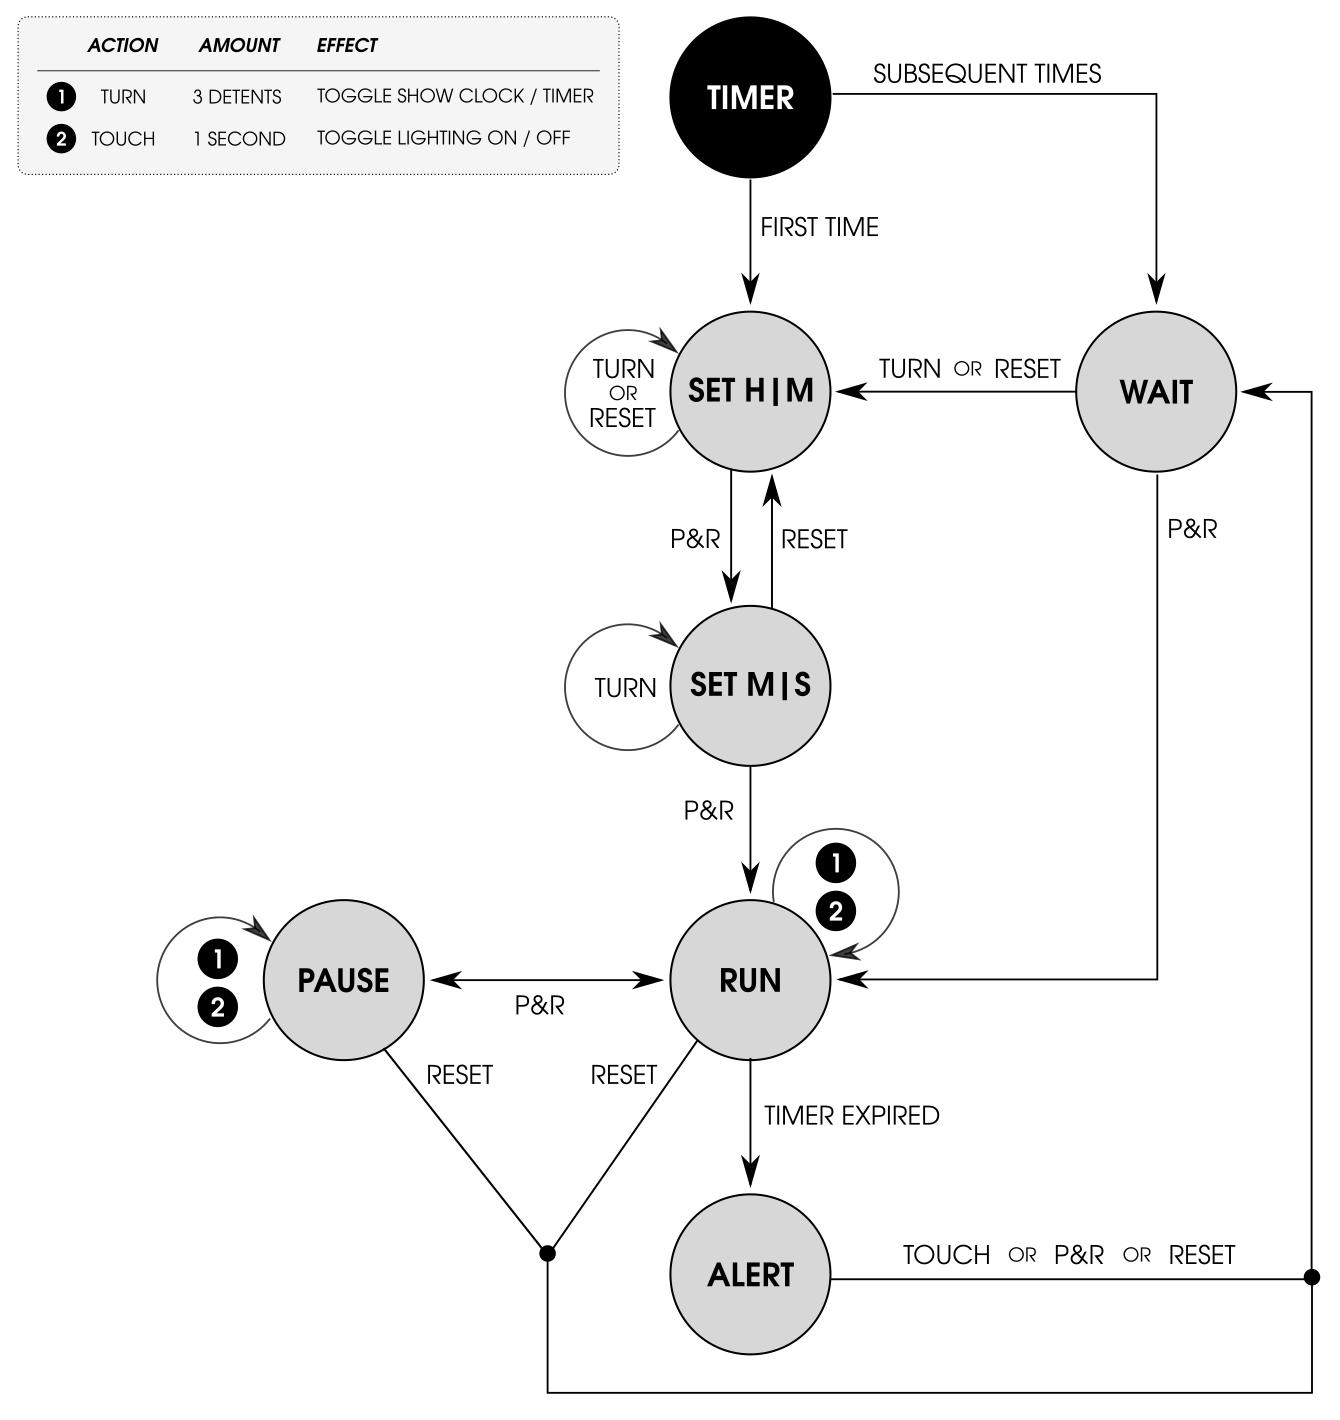
\includegraphics{images/timer_state_diagram.png}
  \caption{Timer - State Diagram}
\end{figure}
